\documentclass[xcolor=dvipsnames]{beamer}
\mode<presentation> {

\usecolortheme{default}
%\setbeamercovered{transparent}

\definecolor{carolina}{HTML}{82CAFA}
%\definecolor{carolina}{HTML}{3BB9FF}
%\definecolor{gray}{HTML}{B6B6B4}
%\definecolor{dark}{HTML}{151B54}

\usetheme{Madrid}
\setbeamercolor{structure}{fg=carolina}
\setbeamercolor{block title}{bg=carolina}
\setbeamercolor{block title example}{bg=carolina}

%Uncomment the following if you prefer for the font color on carolina blue background to be black.
%\setbeamercolor{block title}{fg=black,bg=carolina}
%\setbeamercolor{frametitle}{fg=black}
%\setbeamercolor{title}{fg=black}

\setbeamertemplate{caption}[numbered]
\setbeamertemplate{enumerate items}[circle]
\setbeamertemplate{itemize items}[circle]
\setbeamertemplate{section in toc}[circle]
\setcounter{tocdepth}{1} 
\setbeamercolor{section in toc}{fg=black}

\usefonttheme[onlymath]{serif}

%\setbeamertemplate{footline} % To remove the footer line in all slides uncomment this line
%\setbeamertemplate{footline}[page number] 

% To replace the footer line in all slides with a simple slide count uncomment this line
%\setbeamertemplate{navigation symbols}{}

% To remove the navigation symbols from the bottom of all slides uncomment this line
}

%some commonly used packages
\usepackage{graphics}
\usepackage{graphicx}
\usepackage{tikz}
\usepackage{fancyvrb}
\usepackage{comment}
\usepackage{amsmath}
\usepackage{amssymb}
\usepackage{lipsum}
\usepackage{subcaption}
\usepackage{caption}
\usepackage{comment}
\usepackage{multi row}
\usepackage{copyrightbox}
\usepackage{pdflscape}

\newcommand{\overbar}[1]{\mkern 1.5mu\overline{\mkern-1.5mu#1\mkern-1.5mu}\mkern 1.5mu} %Instead of \bar or \overline, use \overbar for proper length and thickness bar for sample average. 

%Edit the following lump of code to customize with your name, title, and date
\title[Intro to Stats and R]{Statistics and R Computing Workshop Using IBIS Data}
\author[Kevin Donovan]{Kevin Donovan}
\institute[UNC and IBIS]{UNC-Chapel Hill and IBIS Network}
\date[10/22/2020]{10/22/2020}

\newcounter{saveenumi}
\newcommand{\seti}{\setcounter{saveenumi}{\value{enumi}}}
\newcommand{\conti}{\setcounter{enumi}{\value{saveenumi}}}

\resetcounteronoverlays{saveenumi}

\begin{document}

\begin{frame}
	\titlepage
\end{frame}

\section{Introduction}
\begin{frame}
\frametitle{\insertsectionhead}
\textbf{Reproducibility in the Computing Age}
\begin{figure}
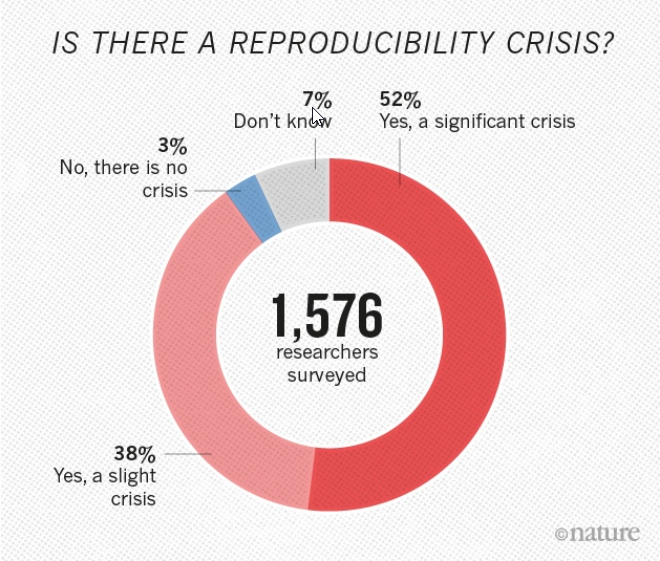
\includegraphics[scale=0.45]{images/reproducibility.png}
\end{figure}
\end{frame}

\begin{frame}
\frametitle{\insertsectionhead}
Evidence shows low reproducibility of scientific research despite
\begin{enumerate}
\item Extensive professional specialization
\item Well-developed methodology for study design and data analysis
\item Explosion in open source statistical software and computing tools
\item Software supported by extensive documentation
\end{enumerate}
\textbf{How can we turn the tide on the reproducibility issue?}
\end{frame}

\begin{frame}
\frametitle{\insertsectionhead}
\textbf{My part}:\\
Principled and detailed statistical consulting and education\\~\\

\textbf{Goals with IBIS}:\\
\textbf{NOT} to:
\begin{enumerate}
\item Teach scientists to be self-reliant statistically
\item Use statistical jargon scientists and expect them to decipher
\end{enumerate}
\textbf{YES} to:
\begin{enumerate}
\item Teach scientists about fundamental statistical methods and concepts
\item Teach scientists good programming practices for data management and visualization
\item Focus less on jargon and more on concepts of statistical analysis
\end{enumerate}
\end{frame}

\section{Welcome}
\begin{frame}
\frametitle{\insertsectionhead}
\textbf{Motivation for class}:\\
Acting on goals for \textbf{whole IBIS network}

\begin{exampleblock}{About Me}
\begin{figure}
\includegraphics[scale=0.6]{../../../../kmdono02.github.io/profile.PNG}
\end{figure}
PhD student in Biostatistics\\
UNC at Chapel Hill\\
Email: kmdono02@ad.unc.edu\\
Basketball and Green Bay Packers enthusiast
\end{exampleblock}
\end{frame}

\begin{frame}
\frametitle{\insertsectionhead}
\textbf{Structure for class}:
\begin{itemize}
\item Lecture and Q+A sessions - 1 hour, twice a month
\item Office Hours - 2 hours, twice a month, open
\item No slides filled with code, \textbf{NO} droning on about coding
\item Focus on \textbf{live and conceptual programming}
\item \textbf{All lectures and code publically available}
\end{itemize}

\begin{figure}
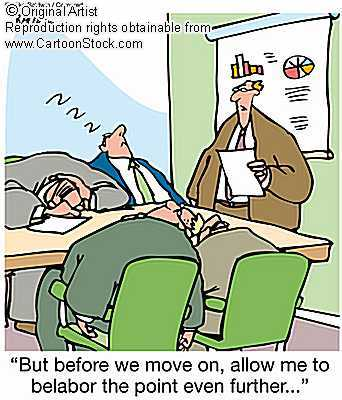
\includegraphics[scale=1.25]{images/boring-lecture.jpg}
\end{figure}

\end{frame}

\begin{frame}
\frametitle{\insertsectionhead}
\textbf{Goals for class}:
\begin{enumerate}
\item Primary: Promote the understanding of statistical concepts and mindset
\item Secondary: Teach tools in R software for
\begin{enumerate}
\item data management
\item data visualization/tabulation
\item exploratory analysis
\item \textbf{reproducibility}
\end{enumerate}
\item Make statistics and coding less intimidating and more exciting!
\end{enumerate}

\end{frame}

\end{document}

